We will be comparing our results with the Infinite Impulse Response (IIR) method 
based on the continued fraction expansion approximation to
$s^\alpha$.~\cite{Chen:04a} Its benefits are that it has a flat phase response over
approximately two and a half decades in phase for a 9th order
expansion (10 registers of input signal memory). It would be desirable
to find an algorithm with an even broader flat phase frequency
bandwidth and with a comparably small amount of memory required. We
take the Gr{\"u}nwald algorithm as a starting point. As the signal history
retained in the Gr{\"u}nwald sum grows longer, the bandwidth of flat phase
response grows broader; however, the memory required also increases
with input signal history length. To reduce this memory requirement
and retain a long signal history, we propose partitioning the input
signal history into bins that are longer further into the past. The
value of the binned input signal is represented by the average value
of the input signal within that bin. The presence of short bins at
recent times maintains sensitivity to high frequencies, while the 
inclusion of long bins at past times adds sensitivity to low frequencies 
that would not be present in a truncated Gr{\"u}nwald 
sum with the same number of terms. (See Figure~\ref{fig:freqScaling}).


\begin{figure}
\centering
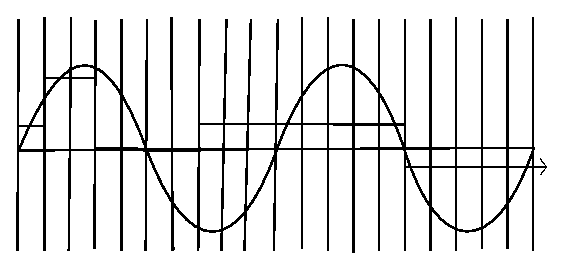
\epsfig{file=FIG1A.eps, height=40mm, width=90mm}
\\a. Higher frequency\\
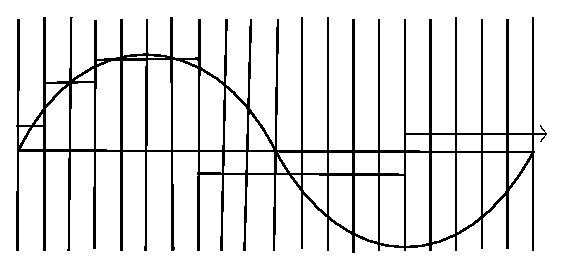
\epsfig{file=FIG1B.eps, height=40mm, width=90mm}
\\b. Lower fequency
\caption{Let each division represent a single time step and each bar represent a bin, scaled such that the duration of a bin increases further back in time (toward the right). The value of the bin is the average of the input signal, the sine wave, at each point in time within that bin. There exists some oldest bin that responds sensitively to the input signal (the second bin for Figure~a and the third bin for Figure~b). Since the time step and binning structure are held fixed, at lower frequencies, the oldest sensitive bin moves to older times (to the right). This illustrates the sensitivity of short bins at recent times to high frequencies and the sensitivity of long bins in the  more distant past to low frequencies. }
\label{fig:freqScaling}
\end{figure}

\begin{table}
Abbreviations and notation used this paper:\\
\begin{tabular}{  l@{ -- } l  p{3.0in}}
IIR & Infinite Impulse Response\\
FO & Fractional Order\\
GL &  Full Gr{\"u}nwald calculation\\
GL\# & Truncated Gr{\"u}nwald calculation to \# terms\\
LIN\# & Linear binning, \# bins\\
SQ\# &  Squared binning, \# bins\\
EXP\# & Exponential binning with a base of two, \# bins\\
FIB\#& Fibonacci binning, \# bins\\
$N_b$ & number of memory bins\\
$N_h$ & full history capacity of the algorithm\\
$N_t$ & number of data items up to time $t$\\
\end{tabular}
\end{table}

\subsection{Modified Gr{\"u}nwald}

The Gr{\"u}nwald form of the fractional derivative of order $\alpha$ can be written~\cite{OldSpan:74}

\begin{equation}
_0D^\alpha_tf(t) = \displaystyle \lim_{N\to\infty} \left(\frac{t}{N_t}\right)^{-\alpha}
\displaystyle\sum\limits_{j=0}^{N_t-1} w_{j}x_j
\label{simpleGrunwald}
\end{equation}
where $f(t)$ is the input signal at time $t$, the $j$th value of the
input signal history is $x_j=f\left(t-\frac{j\Delta t}{N_t}\right)$, and the
$j$th Gr{\"u}nwald weight is

\begin{equation}
w_{j} = \frac{\Gamma(j-\alpha)}{\Gamma(j+1)\Gamma(-\alpha)}.
\label{wj}
\end{equation}
For the purposes of this paper, the order will be constrained $-1<\alpha<1$. Note 
that a fractional order integral is simply a derivative of negative order. Both 
derivatives and integrals are computed over a finite interval. It is assumed
that the system is non-initialized; that is that are no initial conditions.

To include more distant history at low computational cost, we modify
the Gr{\"u}nwald sum of Equation~\ref{simpleGrunwald} by partitioning its
history into $N_b$ bins. In each bin $k$, the input signal history
$x_j$ is represented by its average value over that bin, $X_k$.

Since we make the assumption that each value is well represented by
its average within a bin, we can define a value for the "bin
coefficient" by summing the Gr{\"u}nwald coefficients within that bin.

\begin{equation}
W_k = \displaystyle\sum\limits_{j=p_{k-1}+1}^{p_k} w_j
\label{eqn:sumWk}
\end{equation}

\noindent where $w_j$ is summed from the lowest index of the input data history within bin $k$ to the highest index $p_k$ within that bin. Define
\begin{equation}
N_h=p_{N_b}=\displaystyle\sum_{k=0}^{N_b}b_k
\label{eqn:Nh}
\end{equation}
for later reference. 

With these definitions, the modified Gr{\"u}nwald differ-integral can be written

\begin{equation}
_0D^\alpha_t f(t) = \displaystyle(\Delta t)^{-\alpha}\sum\limits_{k=0}^{N_b}\bar{W}_kX_k
\label{avgSimpleGrunwald}
\end{equation}
where $\Delta t$ is the interval between time samples. There is an additional factor that goes into $\bar{W}$ that will be discussed in Section~\ref{sec:shifting}. Note that in the average Gr{\"u}nwald algorithm, $N_h$ plays the role of the last virtual time element to effectively enter the modified summation, rather than $N_t$. Here, $N_t$ plays the role of the number of time steps that have occurred since the algorithm started to run. 



\subsection{Updating the average history}
\label{sec:shifting}

When a new input data element is read, the history is updated. The new data element is shifted into the first bin through a weighted average. Since data elements represent time steps, they should be incompressible-- when one element is shifted into a bin, another virtual element should be shifted out of that bin if the bin is full. It shifts into the next bin, and pushes a virtual element out of that one, until a bin which is partially full or empty is reached. To update the average data stored in the bins, we take the weighted average obtained by adding one virtual element from the $(k-1)$th bin to the $b_k$ elements in the $k$th bin. This process is illustrated in Figure~\ref{fig:binShifting}.

\begin{figure}
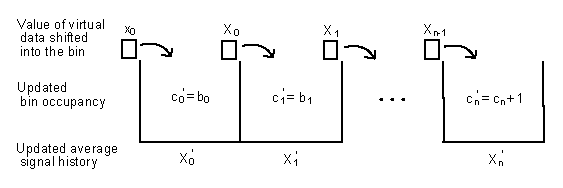
\epsfig{file=FIG2.eps,height=25.5mm,width=90mm}

\caption{When the input data $x_0$ is read, virtual data elements with bin average values $X_k$ are shifted from the $k$th to the $(k+1)$th bin. The first $n-1$ bins are at capacity, but the $n$th bin gains one data point. The bin averages are updated to value $X_k^\prime$ through a weighted average.}
\label{fig:binShifting}
\end{figure}

During start-up, it will be necessary to consider a bin that has some
set size $b_k$, but is not filled to that capacity. In that case, it
is the current occupation number $c_k$ of that bin that enters the
calculation. The algorithm for updating bins can be stated generally if the occupation number of the $k$th bin is defined to be $c_k$. In that case, $c_k=b_k$ for all the bins more recent than the bin that is in the process of filling. No updating occurs for older bins. 

If the $k$th bin initially contains $c_k$ elements,
updating the history either leaves $c_k$ ($c_k^\prime=c_k=b_k$) or
increments the number of elements in the bin such that $c_k^\prime =
c_k + 1$ if the bin is not yet at capacity. Either way, the updated
average of the value of the $k$th bin, $X_k^\prime$, is given by

\begin{equation}
X_k^\prime = \frac{c_k^\prime-1}{c_k^\prime}X_k + \frac{1}{c_k^\prime}X_{k-1}.
\label{eqn:updating}
\end{equation}
where $X_{-1}$ is taken to be $x_0$, the input data that has just been
read. 

During start-up, the partially full bin also factors into
the Gr{\"u}nwald weights. To handle the bin that is partially full, we
weight the binned Gr{\"u}nwald weights by the ratio of the bin occupation
number $c_k$ to its capacity $b_k$,

\begin{equation}
\bar{W}_k= \frac{c_k W_k}{b_k}.
\label{eqn:Wbar}
\end{equation} 







